\begin{figure*}[t]
    \centering
    \begin{tabular}{@{}cccc@{}}
      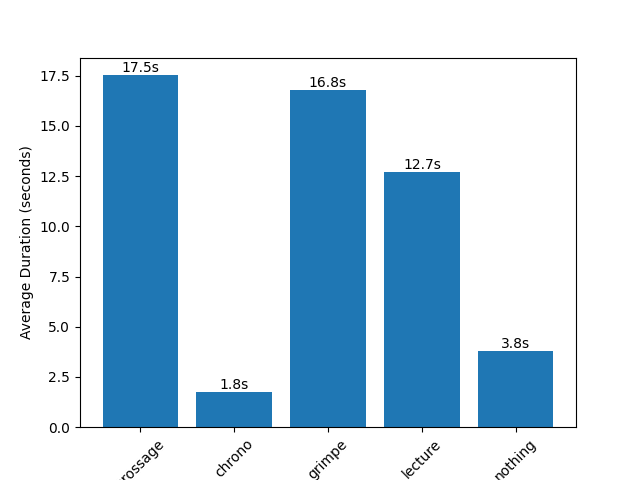
\includegraphics[width=0.23\textwidth]{../../assets/figures/average-duration-of-actions.png} &
      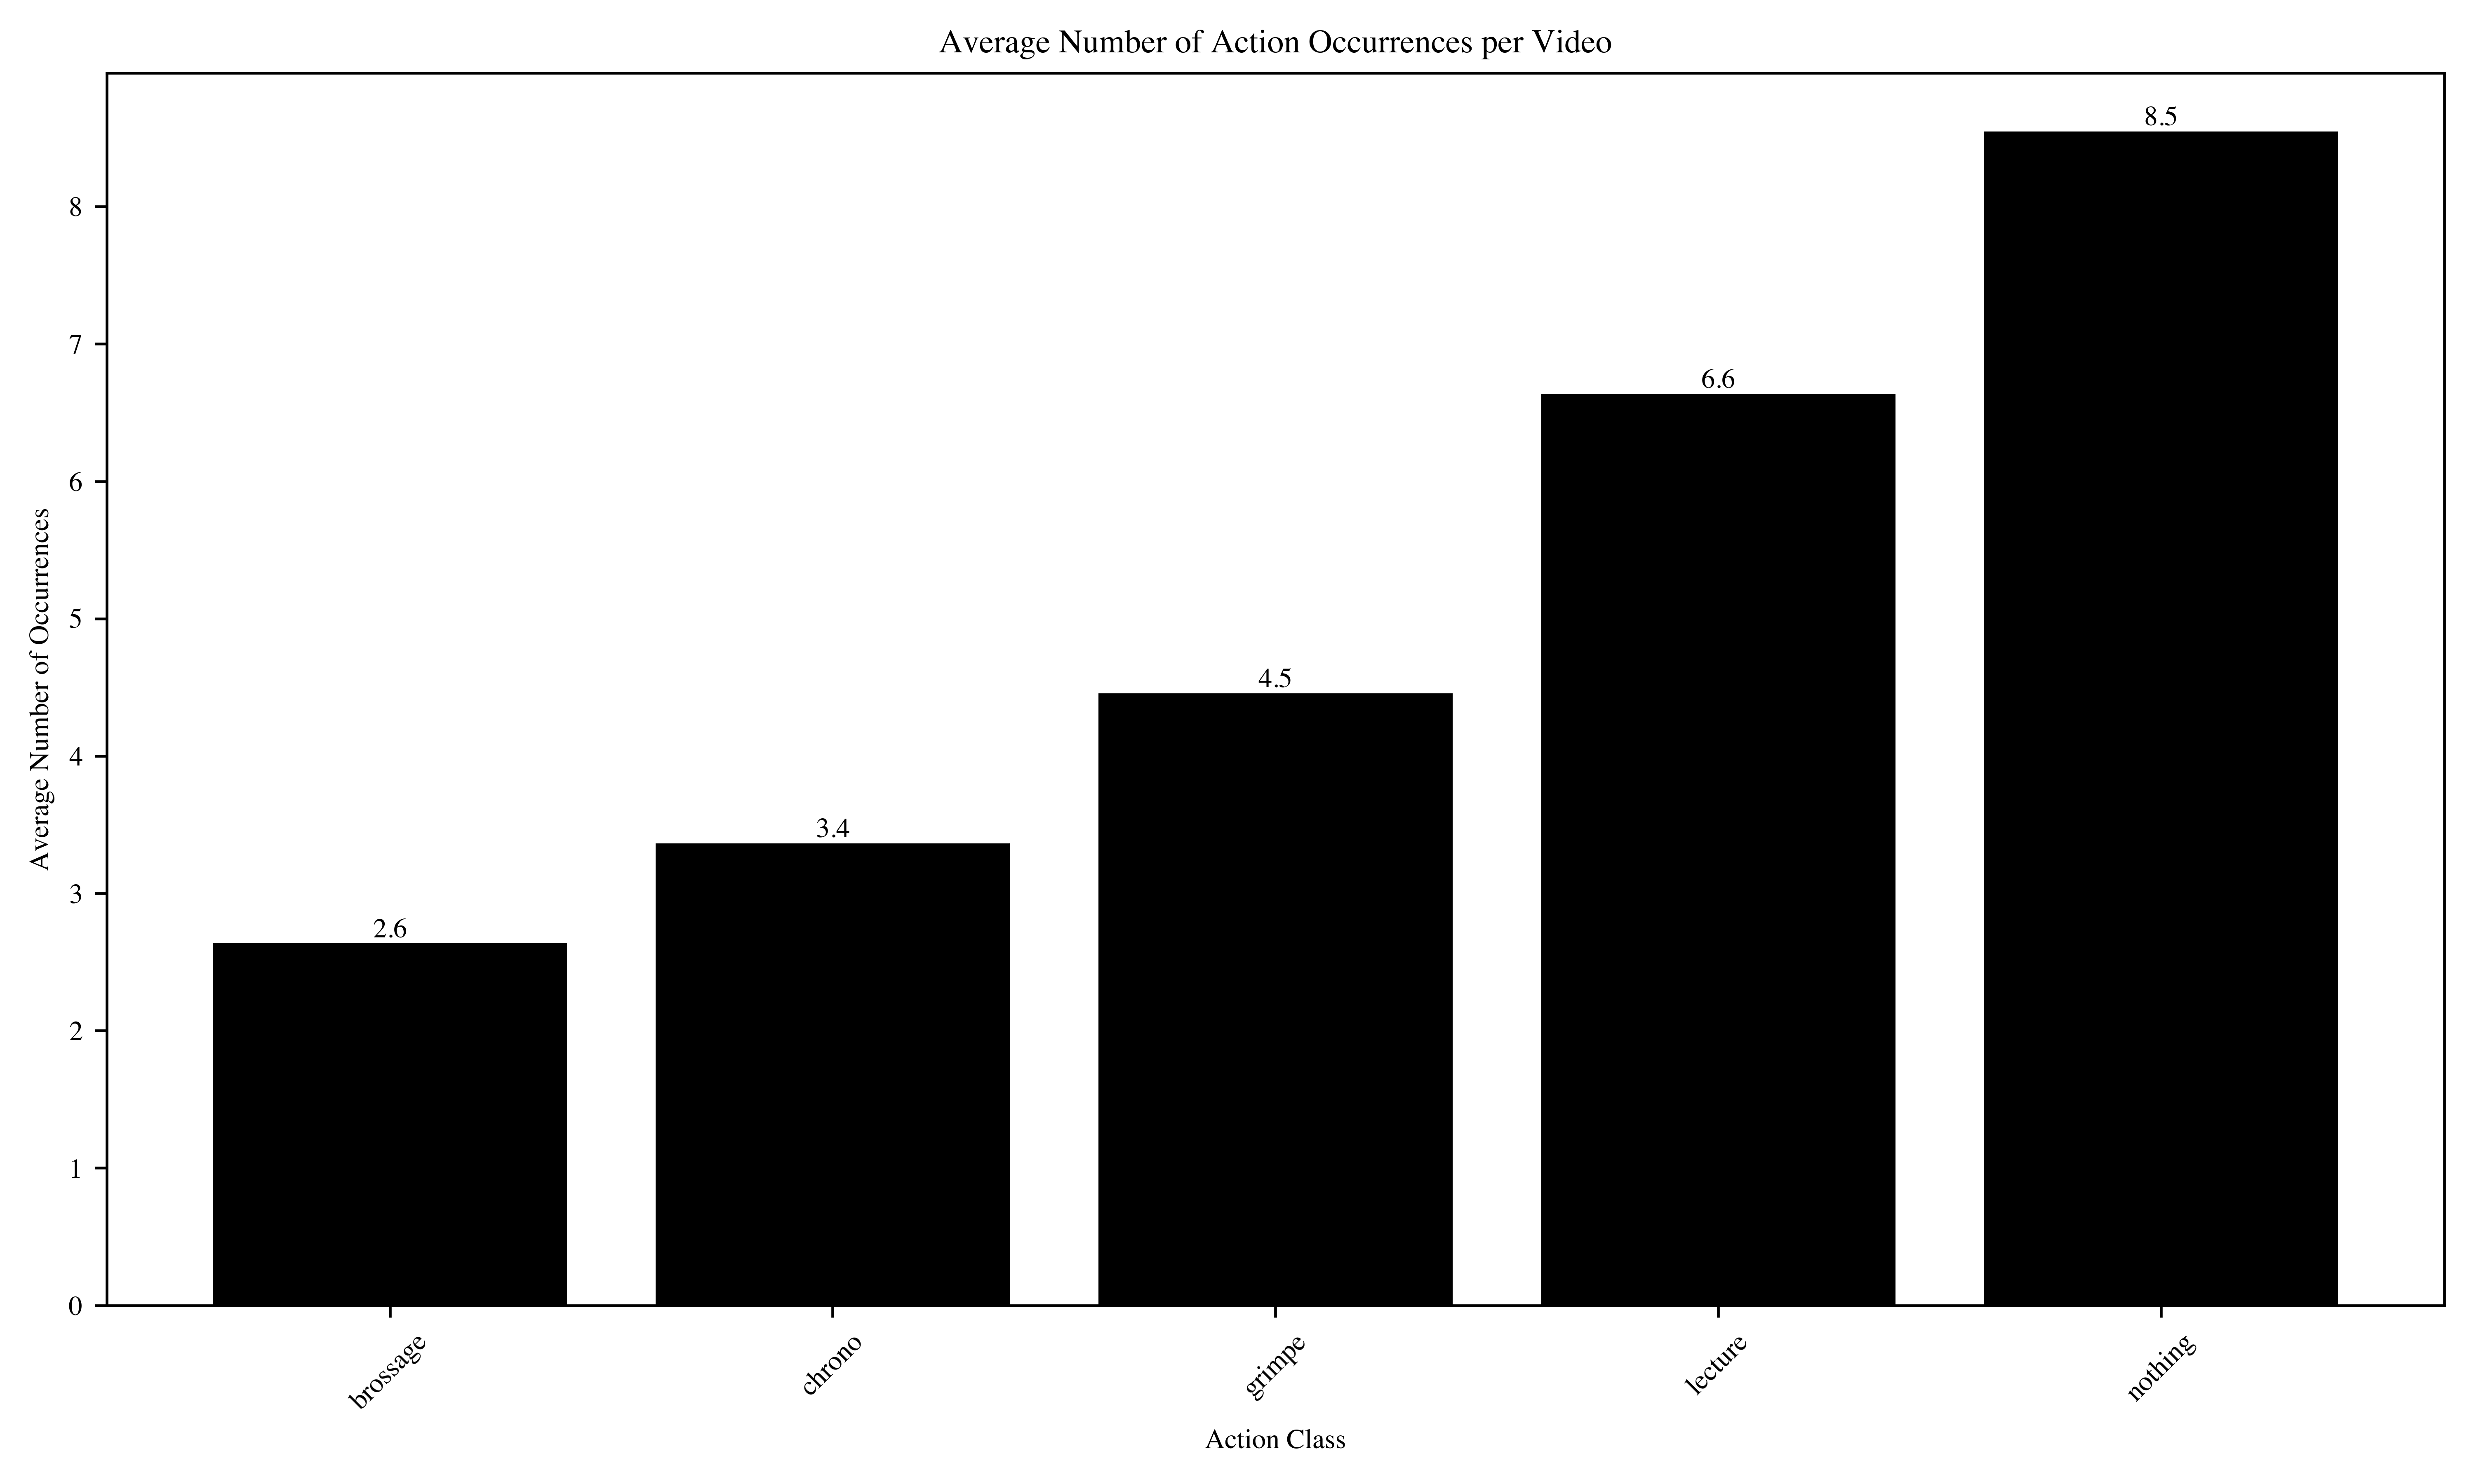
\includegraphics[width=0.23\textwidth]{../../assets/figures/average-number-of-action-occurrences-per-video.png} &
      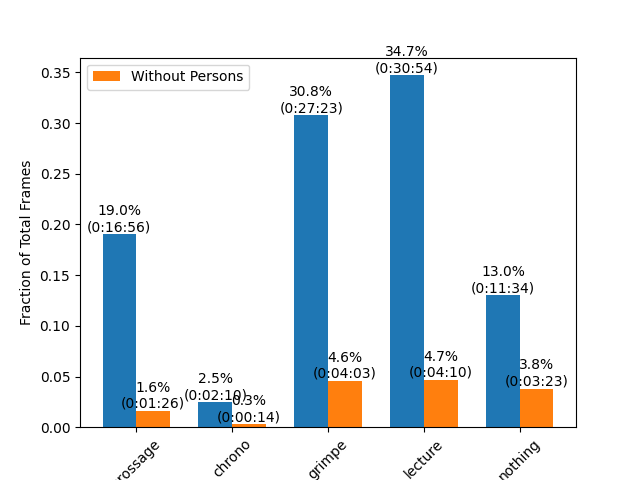
\includegraphics[width=0.23\textwidth]{../../assets/figures/distribution-of-actions-in-dataset.png} &
      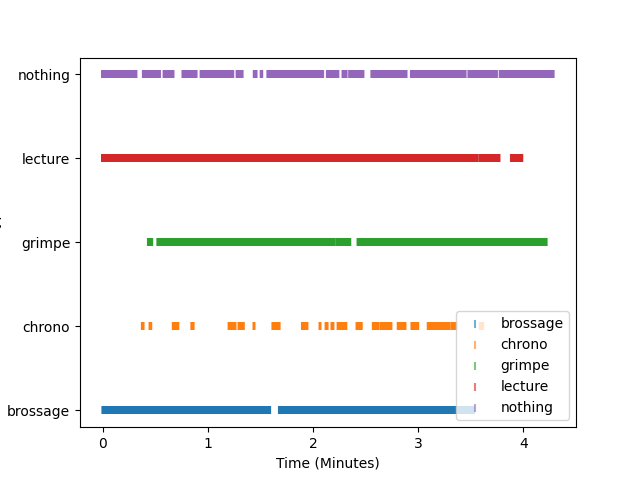
\includegraphics[width=0.23\textwidth]{../../assets/figures/temporal-distribution-of-actions.png} \\
      \begin{minipage}{0.23\textwidth}\centering\caption{Average duration of actions in the dataset.}\label{fig:average-duration-of-actions}\end{minipage} &
      \begin{minipage}{0.23\textwidth}\centering\caption{Average Action Count per Video.}\label{fig:average-number-of-action-occurences-per-video}\end{minipage} &
      \begin{minipage}{0.23\textwidth}\centering\caption{Distribution of actions in the dataset.}\label{fig:distribution-of-actions-in-dataset}\end{minipage} &
      \begin{minipage}{0.23\textwidth}\centering\caption{Temporal distribution of actions in the dataset}\label{fig:temporal-distribution-of-actions}\end{minipage}
    \end{tabular}
  \end{figure*}

\section{Dataset}

In this section, we present our dataset along with the different steps involved in its construction and preparation. We also provide some statistics about the dataset and compare it to other popular datasets.

\subsection{Raw Format}

The dataset was collected during "Manip Chambery" Our dataset was constructed by filming 10 different climbers attempting to climb 2 different bouldering blocks (events) each. Each climb was filmed from two different angles, resulting in 20 climbs and a total of 40 unique videos, each 4 minutes long.

As specified in \cite{section:context}, during the bouldering event, climbers are free to perform various activities within the 4-minute duration. They can brush the holds (grips), observe them, climb, etc.

The videos were annotated by the climbers themselves, and the annotations were provided in a raw Excel file. The annotations are at the segment level, meaning we are provided with the start time and duration of each action in the video, along with the corresponding label. Our of the 20 climbs only 11 have been annotated.

The total duration of our dataset is 2 hours and 40 minutes from which only 1 hour and 28 minutes are annotated.

The dataset has several limitations: \textbf{1.} The dataset size is very limited. \textbf{2.} The annotation format (Excel) is not suited for data science tasks. \textbf{3.} The annotations are not perfect: they are shifted, and the videos do not start immediately with the event. \textbf{4.} The climbers occasionally go out of the frame, and at other times, another person enters the frame.

\subsection{Chosen Structure}

We decided to structure the dataset in a way that is specifically suited for temporal action segmentation and classification tasks. Our main objective was to ensure that it is both easy to use and efficient for training.

\begin{verbatim}
    dataset
    +-- videos
    |   +-- video-1
    |   |   +-- frame-1.jpg
    |   |   +-- frame-2.jpg
    |   |   +-- ...
    |   +-- ...
    +-- annotations
    |   +-- video-1.csv
    |   +-- video-2.csv
    |   +-- ...
\end{verbatim}

The advantage of this structure is that it does not require any additional processing of the videos or annotations provided by the data collection team. This makes it convenient and easy to add new annotations or videos in the future, should they become available.

For faster video loading, we store the videos as a sequence of JPG frames instead of the video file itself. This approach also facilitates the use of the dataset with different libraries and tools.

To load the dataset, we developed a Python package: \href{https://github.com/raideno/video-dataset}{https://github.com/raideno/video-dataset}. This package supports this type of dataset structure but is highly customizable and includes many predefined tools for transforming an existing dataset into this format, loading videos from video files, and loading annotations at the frame level from text files.

Additionally, we developed another Python package: \href{https://github.com/raideno/cached-dataset}{https://github.com/raideno/cached-dataset}, which serves as a wrapper around an existing dataset and caches the transformed version of the dataset to disk. This is particularly useful to avoid re-extracting features each time we train the model or run an epoch.

By using this structure and these tools, we were able to easily load the dataset and start training the model.

\subsection{Data Exploration}

In this section we are going to explore various aspects and statistics about our dataset.

As the plot in Figure \ref{fig:distribution-of-actions-in-dataset} shows, the dataset contains 5 different actions, with each action occurring a different number of times. The distribution of actions is not uniform, with some actions appearing more frequently than others. This non-uniform distribution can be challenging for the model to learn, as it may lead to biases in the predictions. The dataset is unbalanced

We can also see that a significant portion of the dataset (15\%) frames don't contain any person in the frame. We can also observe that 3\% of the time there is more than one person in the frame which can be a source of noise for the model.
In addition to that we can see that 13\% of the climbs are not annotated at all and we thus replaced it by a "Nothing" label.

From \ref{fig:average-number-of-action-occurences-per-video} we  can see that the most recurrent actions are "Lecture" and "Nothing".

From the \ref{fig:average-duration-of-actions} we can see that the longest actions on average are the cleaning, climbing and observation. Even tho the nothing class is the most recurrent it is the shortest in duration on average.

\todo[inline]{Add a fourth plot about the dataset.}

\subsection{Popular Video Datasets}

\label{subsection:popular-video-datasets}

\begin{figure}[h!]
    \centering
    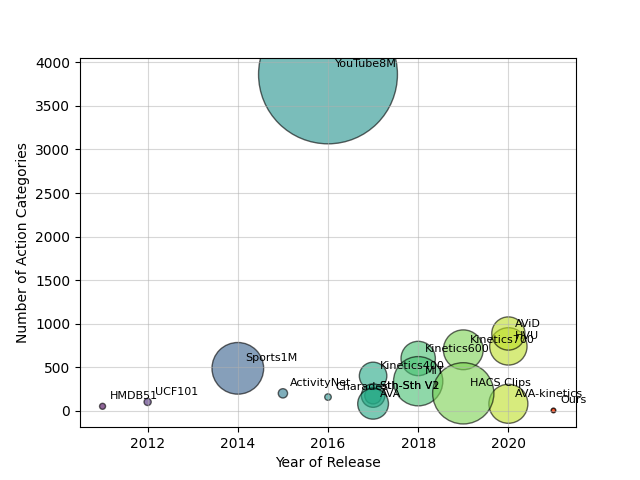
\includegraphics[width=1\linewidth]{../../assets/figures/popular-datasets.png}
    \caption{A visualization of popular video datasets.}
    \label{fig:your-label}
\end{figure}

\begin{table}[!h]
    \centering
    \small
    \resizebox{1\linewidth}{!}{
    \begin{tabular}{lcrr}
    \toprule
    Dataset & Release Year & \#Samples & \#Actions \\
    \midrule
    HMDB51 & 2011 & 7000 & 51 \\
    UCF101 & 2012 & 13300 & 101 \\
    Sports1M & 2014 & 1100000 & 487 \\
    ActivityNet & 2015 & 28000 & 200 \\
    YouTube8M & 2016 & 8000000 & 3862 \\
    AVA & 2017 & 385000 & 80 \\
    \multicolumn{1}{c}{\vdots} & \multicolumn{1}{c}{\vdots} & \multicolumn{1}{c}{\vdots} & \multicolumn{1}{c}{\vdots} \\
    MIT & 2018 & 1000000 & 339 \\
    HACS Clips & 2019 & 1550000 & 200 \\
    HVU & 2020 & 572000 & 739 \\
    AViD & 2020 & 450000 & 887 \\
    \midrule
    \textbf{Ours} & 2024 & 22 & 4 \\
    \bottomrule
    \end{tabular}
    }
    \vspace{-2ex}\caption{A list of popular video datasets.}
    \end{table}

When it comes to temporal action segmentation, there are very few datasets available, and the most popular ones are:

\subsection*{50 Salads, Breakfasts, and GTEA Datasets}
These datasets were primarily designed for temporal action segmentation:

\subsection*{50 Salads, Breakfasts, and GTEA Datasets}
These datasets were primarily designed for temporal action segmentation:

\textbf{1. 50 Salads Dataset}: The 50 Salads dataset consists of 50 videos of people preparing salads, with each video lasting between 5 and 10 minutes. The dataset includes 17 distinct actions, with a total duration of 4 hours. The cameras are placed above the kitchen countertop, capturing primarily the interactions of the person's hands with the environment. This setup focuses on fine-grained actions and interactions \cite{50salads-dataset}.

\textbf{2. GTEA Dataset}: The GTEA dataset was introduced in \cite{gtea-dataset}, and it consists of 28 Point of View (POV) videos, where a person is preparing something. Each video contains around 20 sub-actions.

\textbf{3. Breakfasts Dataset}: Introduced in \cite{breakfast-dataset}, this dataset contains 1712 videos of people preparing breakfasts, with the camera positioned on the side.

\subsection*{Kinetics Family}
The Kinetics family of datasets is available in three variants: Kinetics-400, Kinetics-600, and Kinetics-700 \cite{kinetics-400-dataset}, \cite{kinetics-600-dataset}, \cite{kinetics-700-dataset}. These datasets are composed of YouTube videos and are annotated with 400, 600, and 700 action classes, respectively. The videos typically last around 10 seconds, and each class contains at least 400 videos. The Kinetics datasets cover a wide variety of video content, focusing on humans performing large-scale tasks (as opposed to fine-grained actions). Originally designed for video classification, Kinetics contains single-labeled video clips.

\subsection*{Assembly101 Dataset}
The Assembly101 dataset, introduced in \cite{assembly101-dataset}, contains 4321 videos of people assembling and disassembling various objects in a factory setting. The cameras are positioned at multiple angles, and some videos are captured from a POV perspective.

\subsection*{HowTo100M Dataset}
Introduced in \cite{howto100m-dataset}, the HowTo100M dataset consists of over 100 million video clips sourced from YouTube and other online platforms. It is a collection of instructional (tutorial) videos covering 23,000 distinct activities.

\subsection*{Something-Something V2}
The Something-Something-V2 dataset, introduced in \cite{something-something-dataset}, includes 220,847 video clips of humans performing basic actions such as picking up a pen. The videos are captured from a POV perspective and are designed for fine-grained action and small interaction tasks.